\section{Research questions and OpenMAIC mechanisms}
This chapter tests whether explicit roles, executable evidence, and persistent learner records can turn a weak educational language model into a verifiable tutoring workflow. The evaluation separates the complete system from its model: successful retrieval or a correct fallback is not evidence of autonomous model teaching. The questions concern orchestration, use of learner evidence across turns, and the mechanisms behind successful and failed teaching requests.

The source analysis uses official OpenMAIC commit \texttt{5bd8cc840ee63}, retrieved on 6 November 2026~\cite{openmaic}. The full identifier, permanent links, and SHA-256 checksums of 19 archived files are in \path{tutor/legacy/research/source_manifest.json}. OpenMAIC itself was not deployed; the Python implementation is an independent simplification. Four mechanisms inform the design:

\begin{table}[htbp]\centering\small
\caption{OpenMAIC mechanisms and pinned source anchors. Paths are relative to the pinned upstream repository; permanent links remain in the source manifest.}\label{tab:concise-agents-source}
\begin{tabularx}{\linewidth}{@{}p{25mm}Yp{65mm}@{}}\toprule
Mechanism & What the source actually implements & Source anchors\\\midrule
Roles and scheduling & Teacher, assistant, and classmates have different prompts/actions. A Director selects speakers with \texttt{call\_agent}; useful roles, not fixed round-robin turns, are requested. Child roles can share one model object. Ending actions check that a visible/substantive response exists. & \path{registry/built-in.ts}:12--155; \path{pi/director-loop.ts}:95--221; \path{pi/tools/call-agent.ts}:735--757, 847--864.\\
Course state and evidence & Material analysis/research precede outline and scene generation. Completed steps are explicit state. \texttt{read\_scene} supplies page evidence to subsequent role calls, limiting unsupported guessing. & \path{generation/run/plan.ts}:45--103; \path{generation/src/scene-builder.ts}:21--116; \path{pi/tools/read-scene.ts}:97--124.\\
Context and memory & Child history retains 12 messages. Director compaction preserves goals and unresolved work. PBL Instructor compresses history above 30 messages toward the latest 16, extracts learner clues, and reloads \texttt{earlierSummary}; 4500 characters is its summary-compression threshold. & \path{pi/prompts.ts}:558--589; \path{pi/director-compaction.ts}:95--101, 136--217; \path{v2/agents/instructor-memory.ts}:22--138.\\
Feedback and fallback & Quiz state differs before/after submission. Submitted answers, references, scores, and comments guide feedback. Unparseable model grading can fall back to half credit, which preserves interface operation rather than proving answer correctness. & \path{summarizers/state-context.ts}:172--240; \path{api/quiz-grade/route.ts}:56--105.\\\bottomrule
\end{tabularx}
\end{table}\FloatBarrier

OpenMAIC therefore has more than chat history: it includes scene state and explicit learner-summary mechanisms. However, keyword-derived progress clues are not verified mastery measurements. The project retains role separation, shared evidence, and explicit control while replacing broad multimedia classroom interaction with executable Python-output tasks. It does not reproduce speech, whiteboards, or a complete course editor.

\section{Implementation and verifiable learner memory}
The controller sequentially calls a planner, teacher, and reviewer. Roles share one loaded model, initially the Chapter 2 SFT adapter; later deployments use genuine cloud SFT checkpoints or a separately identified official Instruct model. No weights are updated in this chapter. Planning proposes focus/strategy; teaching returns answer, feedback, explanation, and optional \texttt{followup\_code}; review returns \texttt{approved} and a reason. Actual prompts are Chinese. Complete templates and every executed context, raw response, token identifier, stop reason, and adoption decision remain in the evidence files.

A bounded AST interpreter computes program output and traces. Generated text is not passed to unrestricted \texttt{eval}/\texttt{exec}. The evaluator separately executes reviewed, frozen references in CPython; unsupported programs cannot inherit a reference answer as if verified. Original adoption checks cover the answer, required explanation/feedback text, reviewer approval, and executable follow-ups. Revised controllers add explicit student-status, factual-evidence, and requested code-modification contracts; these stronger checks were absent from the historical C08 run. These gates do not prove all natural-language explanations. Rejected drafts are preserved, and the final response explicitly identifies tool/template fallback.

Original CPU inference uses float32, six threads, greedy decoding, 256 new tokens per role, and a 4096-token input-plus-generation boundary that raises an error rather than silently truncating history. Revised role budgets are 64/192/96. The implementation, model, prompts, and budget of each run are separately frozen.

\begin{figure}[htbp]\centering
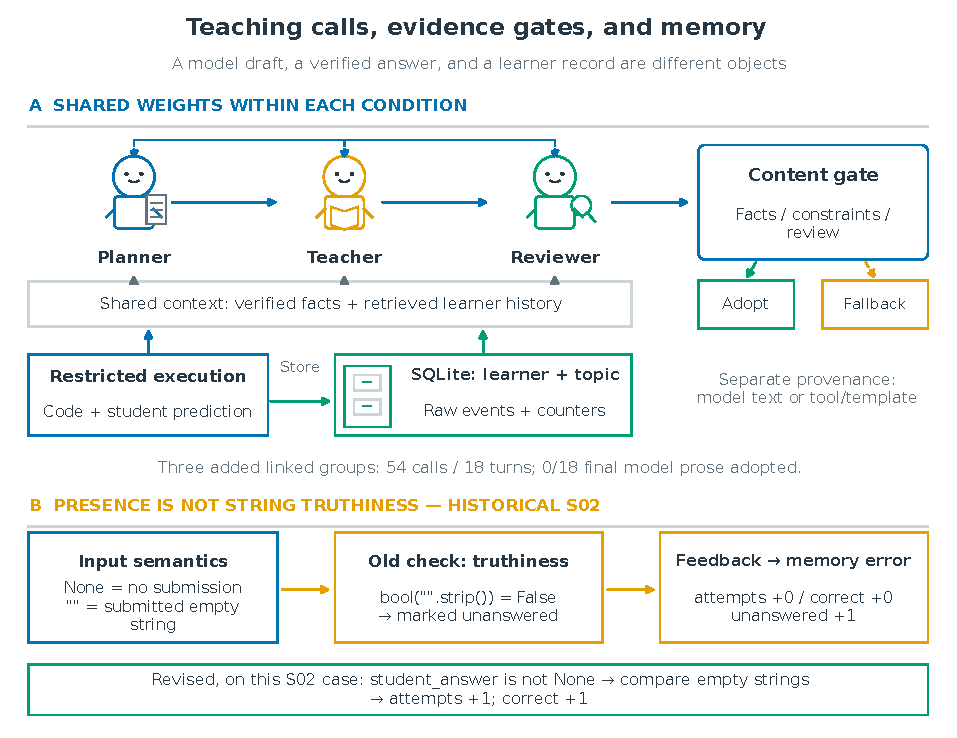
\includegraphics[width=\linewidth]{../../assets/en/teaching-memory.pdf}
\caption{Shared model, role-specific calls, independent evidence checks, and learner memory. The historical empty-string bug is distinguished from its subsequent repair. Friendly role icons explain responsibilities; they are not independently trained models.}\label{fig:concise-agents-system}
\end{figure}\FloatBarrier

SQLite stores raw episodes and derived counters. Episodes retain learner identifier, topic, program, prediction, evidence, role outputs, and final response. Counters distinguish interactions, submitted attempts, correct, incorrect, unanswered, and unverified events. A transaction writes both layers; duplicate event identifiers cannot increment counts twice. Model answers are never counted as student attempts. For learner $u$, topic $k$, and structural difficulty $d$, let $v_t$ indicate verified execution, $a_t$ submitted prediction, and $z_t$ agreement with verified output:
\begin{equation}
N_{u,k,d}\leftarrow N_{u,k,d}+v_ta_t,\qquad
C_{u,k,d}\leftarrow C_{u,k,d}+v_ta_tz_t.
\end{equation}
These are descriptive counts, not calibrated mastery probabilities. The historical approximation of $a_t$ by nonempty text is tested in S02 below.

Retrieval matches the caller-supplied learner ID and topic and supplies the latest three episodes. This assumes a trusted caller; ID filtering is not authentication. Reconstructing the system object reads the same database. Difficulty advice examines recent verified predictions at the same structural difficulty among the latest 100 relevant events, explicitly including the current answer: three consecutive correct predictions suggest an increase; two incorrect suggest a decrease; otherwise it holds. Actual exercise difficulty is checked separately. Exact topic keys, restricted syntax, and uncalibrated thresholds limit personalization; synonym resolution, prerequisites, and forgetting are unimplemented.

\section{Historical protocol and four complete case studies}
The core batch freezes eight scenarios/11 turns; after observing it, a supplementary batch freezes four scenarios/six turns. References include 22 core and 12 supplementary programs/follow-ups executed independently. Complete success requires every necessary automatic check and every predeclared qualitative item to pass. Codex technical review retains textual evidence; it is not blinded teacher assessment. Supplementary design deliberately extends coverage, with implementation hidden from its designer but original cases/results available. It is neither a random sample nor an entirely external blind test.

Together, 12 scenarios produce seven complete and five incomplete tasks, 145/150 automatic checks, and 51 real role calls. No role response is adopted; all 17 final responses use tools/templates. C03/C04 exceed frozen partial-completion expectations. C08/S02 fall below their respective frozen full-completion expectations. C07 remains an expected limitation and is not relabelled. The frozen C03 rationale mentioned earlier ``range/pairing'' errors, but the training study did not actually test range generation; this is retained as a cross-concept risk conjecture, not an observed prior range failure.

\begin{figure}[htbp]\centering
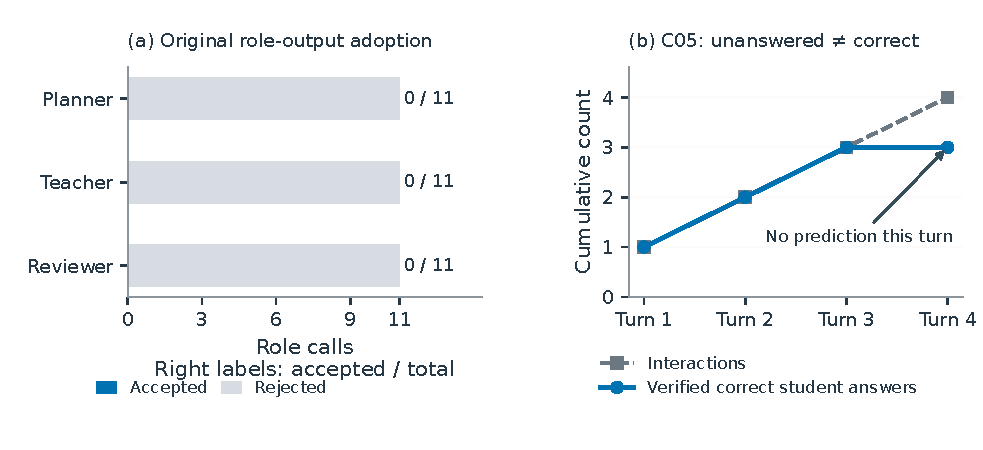
\includegraphics[width=\linewidth]{../../assets/en/agents-evidence.pdf}
\caption{Historical observations: zero accepted role outputs across 11 core turns; in C05, a fourth interaction without a prediction does not increase the three correct attempts. Automatic bookkeeping and pedagogical completeness are different criteria.}\label{fig:concise-agents-evidence}
\end{figure}\FloatBarrier

All quoted responses below are \emph{English translations of recorded Chinese excerpts}, not new English model generations. Complete tasks, references, raw role outputs, final responses, and hashes remain in \path{tutor/legacy/results/core/}, \path{tutor/legacy/results/supplement/}, and \path{reports/case-study-evidence.en.json}.

\Needspace{18\baselineskip}
\subsection{C03: retrieving an earlier mistake across instances}
\paragraph{Task and reference.}
The learner previously included endpoint 8 in \texttt{range(2,8,2)}, predicting 20 rather than 12. After reconstructing the system object, the learner predicts 9, asks for feedback linked to the old mistake, and requests a supplied same-concept follow-up:
\begin{verbatim}
total = 0
for n in range(3, 9, 3):
    total += n
print(total)
\end{verbatim}
The correct result is $3+6=9$, excluding endpoint 9. Changing the endpoint to 12 in the supplied follow-up gives $3+6+9=18$.

\Needspace{12\baselineskip}
\paragraph{Actual response and interpretation.}
The raw teacher repeats instructions about checking misconceptions, fails the structured contract, and is rejected. The final response includes:
\begin{quote}\small
Your previous prediction on this concept was \texttt{'20'}; the verified output was \texttt{'12'}. Your words were ``I included 8 as well, so I guessed 20.'' This is answer evidence, not a mastery conclusion.

Output: 9. Your current prediction agrees with execution. \texttt{range(3,9,3)} takes \texttt{[3,6]}; endpoint 9 is excluded. Follow-up reference output: 18.
\end{quote}
Two predictions remain in the database, one correct and one incorrect. This exceeds the partial expectation because retrieval survives object reconstruction and preserves old evidence. The quote comes from deterministic database access and the explanation from execution traces, not demonstrated model reasoning about learner history.

\Needspace{17\baselineskip}
\subsection{C04: separating a new learner on the same topic}
\paragraph{Task and reference.}
A different learner provides no prediction, requests explanation and the supplied follow-up, and must not inherit the previous learner's history:
\begin{verbatim}
total = 0
for n in range(2, 8, 2):
    total += n
print(total)
\end{verbatim}
The original result is $2+4+6=12$. The supplied follow-up changes the endpoint to 10, giving $2+4+6+8=20$. Submitted and correct counts should remain zero.

\Needspace{10\baselineskip}
\paragraph{Actual response and interpretation.}
The raw teacher repeatedly lists execution-step and follow-up instructions without a usable response. Final tool/template feedback states:
\begin{quote}\small
Output: 12. No prediction was provided, so this is not recorded as a correct or incorrect answer. \texttt{range(2,8,2)} takes \texttt{[2,4,6]}; endpoint 8 is excluded. Follow-up reference output: 20.
\end{quote}
Retrieval is empty. After writing, the new learner has one interaction, zero attempts, and one unanswered event. No old student's misconception is cited. This exceeds the partial expectation and verifies identity-scoped retrieval for this input, not deep adaptation to different learning backgrounds.

\Needspace{21\baselineskip}
\subsection{C08: correct execution but an invalid constrained follow-up}
\paragraph{Task and reference.}
The learner predicts 230 and asks for paired contributions, the unpaired element, and a follow-up created \emph{only by appending one number to the right list}. The task program and actually delivered follow-up are shown together:
\par\noindent\begin{minipage}[t]{0.48\linewidth}\small
\textbf{Task program}\par
\begin{verbatim}
left = [9,24,17,32,6,18]
right = [7,16,35,22,44]
total = 0
for a, b in zip(left, right):
    total += a + b
print(total)
\end{verbatim}
\end{minipage}\hfill
\begin{minipage}[t]{0.48\linewidth}\small
\textbf{Actual delivered follow-up}\par
\begin{verbatim}
left = [9,24,17,32,6,18]
right = [7,16,35,22,44]
total = 1
for a, b in zip(left, right):
    total += a + b
print(total)
\end{verbatim}
\end{minipage}\par
Five pairs contribute $16,40,52,54,50$, totaling 212; left-tail 18 is unpaired. Appending 6 to the right list is one valid reference, yielding $212+18+6=236$. Other appended values are valid when the program and explanation agree.

\Needspace{9\baselineskip}
\paragraph{Actual response and root cause.}
The unstructured raw teacher response is rejected. The final response correctly gives 212 and its pair contributions, but then says:
\begin{quote}\small
Follow-up: change only the 0 on original line 3 to 1; leave everything else unchanged. Follow-up reference output: 213.
\end{quote}
The delivered code really outputs 213 but changes the accumulator rather than the right list; it still has five pairs. All five original automatic checks pass. The missing contract is whether the edit satisfies the teaching request, not executability. This is below the frozen full expectation and is the original batch's genuine unexpected failure.

\Needspace{20\baselineskip}
\subsection{S02: a correct empty-string prediction becomes unanswered}
\paragraph{Task and reference.}
The learner explicitly submits \texttt{student\_answer=""} and says ``my prediction is an empty string, meaning one printed blank line.'' The original and supplied follow-up are
\begin{verbatim}
word = 'python'
print(word[4:1])   # Original
word = 'python'
print(word[1:4])   # Supplied follow-up
\end{verbatim}
The default positive step selects no indices in \texttt{[4:1]}. CPython emits exactly one newline; normalization leaves an empty string, matching the prediction. Attempts and correct answers should each increase once, with unanswered unchanged. The follow-up reference is \texttt{yth}.

\Needspace{12\baselineskip}
\paragraph{S02 recorded response and root cause.}
The raw teacher wrongly claims the original slice returns \texttt{python} and is rejected. The final response instead begins with a genuinely blank output field:
\begin{quote}\small
Output:

No prediction was provided, so this is not recorded as correct or incorrect. \texttt{word[4:1]} selects indices \texttt{[]} and gives \texttt{''}. Follow-up reference output: \texttt{yth}.
\end{quote}
Nothing follows the first colon in the recorded field. The interpreter and follow-up are correct, but feedback and SQLite label the submitted prediction \texttt{unanswered}; attempts/correct remain zero and unanswered increases once. Only 5/9 checks pass. The condition \texttt{bool(student\_answer.strip())} conflates valid empty content with no submission before comparing answers. This distinct state-representation failure falls below its supplementary batch's frozen full expectation, providing the second unexpected failure without changing C07's label.

\begin{figure}[htbp]\centering
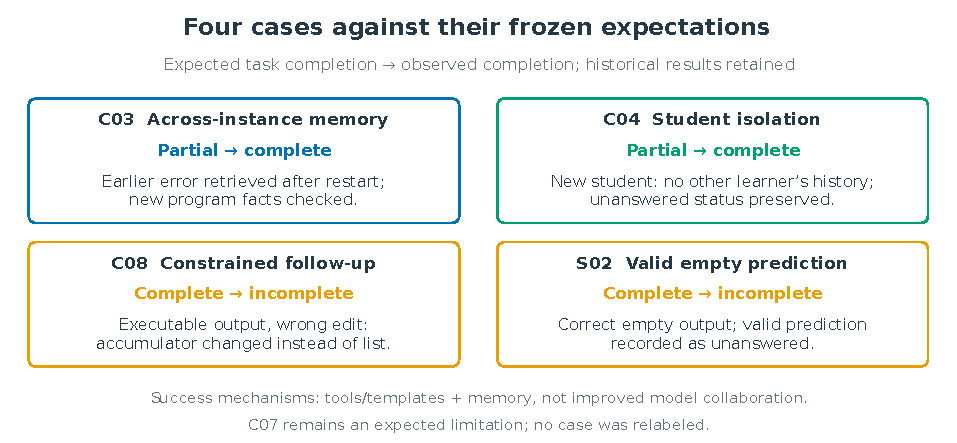
\includegraphics[width=\linewidth]{../../assets/en/case-outcomes.pdf}
\caption{Four historical cases against their own pre-run expectations. C03/C04 successes rely on verified records and templates; C08/S02 reveal different controller defects. Later repairs do not erase original outcomes or convert them into new successes.}\label{fig:concise-agents-cases}
\end{figure}\FloatBarrier

\section{Repairs, controls, and model-linkage results}
Repairs are isolated under \path{tutor/core/}; original inputs, databases, files, expectations, and labels remain unchanged. Known-case regression is not an unseen test. Fourteen unit tests additionally cover negation, edit scope, output whitespace, erroneous states, and learner separation; scripted backends are unit-test-only.

C07's missing exercise arose from a 12-character request window facing a 16-character gap. The revised detector removes that window and checks negation; bounded empty-list/dictionary default repairs use \texttt{None} and entry-time allocation. C08 now requires that removing the newly appended right-list element recover the original AST. Appending 1 yields 231, a legitimate alternative to the 236 reference. S02 distinguishes \texttt{None} from submitted empty text and removes only one trailing newline. Corrected counts are attempts +1, correct +1, unanswered +0. The first repaired tool card wrongly treats the default-expression list \texttt{[None]} as a mutable default, although the actual parameter default is \texttt{None}; the later common pipeline checks default type and entry AST and corrects that explanation. Correct code alone did not validate its teaching text.

\begin{table}[htbp]\centering\small
\caption{Controller and memory controls. Adopted text is not a teaching-quality score.}\label{tab:concise-agents-controls}
\begin{tabularx}{\linewidth}{@{}Yrrrr@{}}\toprule
Configuration & Turns & Calls & Final adoption & Checks\\\midrule
Tools/templates, memory on &17&0&0&209/209\\
Same system, memory reading off &17&0&0&204/209\\
Official Instruct, multi-role &17&51&1&209/209\\
Official Instruct, single-role subset &6&6&1&70/70\\\bottomrule
\end{tabularx}
\end{table}\FloatBarrier

The memory control still writes audit events but loses three retrieval checks (C03/S03/S04) and C05's difficulty advice/delivery checks. This supports those mechanisms, not model memory reasoning or learning gains. The external official Instruct checkpoint is not a substitute for the project's trained SFT. Thirteen of 17 raw teachers copy a numeric prompt example; all 17 reviewers approve even faulty drafts. Only C03 passes outer gates, by repeating the supplied F1 tool card verbatim. On the same six cases, single-/multi-role teacher and final texts are identical; calls are 6 versus 18 and generation times approximately 35.0 versus 73.5 seconds, without an observed final-response gain.

\begin{table}[htbp]\centering\small
\caption{Prompt/evidence diagnostics on the same eight new, prospectively frozen challenges. Tasks were informed by earlier faults. Fence compatibility was added after seeing same-task outputs and is exploratory.}\label{tab:concise-agents-prompt}
\begin{tabularx}{\linewidth}{@{}Yrrrr@{}}\toprule
Condition & Calls & Teacher parsed & Final adoption & Checks\\\midrule
No examples, free explanation &24&8/8&1/8&64/64\\
No examples, bare-JSON strict quotation &24&0/8&0/8&64/64\\
Complete-fence compatibility retest &24&8/8&1/8 quote&64/64\\\bottomrule
\end{tabularx}
\end{table}\FloatBarrier

Free explanation matches 7/8 answer fields but only 2/8 student states; its sole adoption is generic tool commentary. The strict condition's fenced raw texts manually match 7/8 answers and 3/8 states, but formal bare-JSON parsing remains zero. Complete-fence compatibility restores parsing without fixing these states; seven reviewer approvals still conflict with content requirements. Only P03 adopts \emph{model-selected tool evidence}, not independent free explanation. Raw teacher outputs are identical to the preceding strict condition; reviewer inputs change after parsing, so this is a real pipeline rerun, not offline parsing counted as new model reasoning. Exploratory pairing on the old six tasks uses 18 calls per prompt condition: free explanation adopts 2/6 but one overclaims understanding from a single correct prediction; strict quotation parses/adopts zero. Both pass 70/70 through verification and fallback. Prompt, controller, and tool-card changes occur together and are not a prompt-only ablation.

\begin{figure}[htbp]\centering
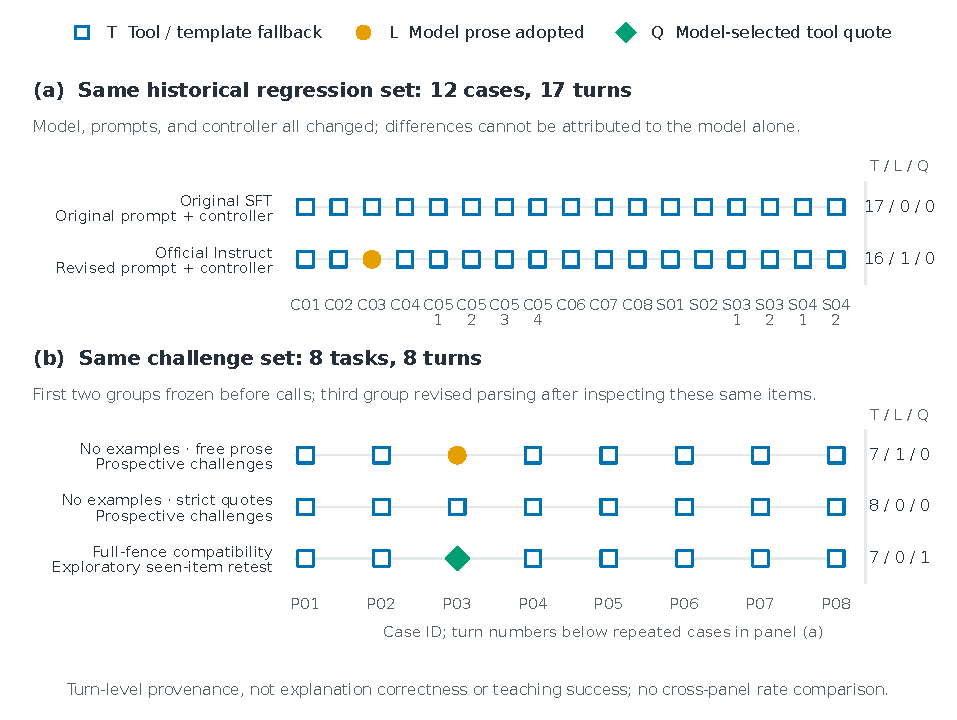
\includegraphics[width=\linewidth]{../../assets/en/agents-revision-provenance.pdf}
\caption{Recorded final-content sources: template/tool fallback, adopted model prose, and model-selected tool quotation. Panels use different task sets; no cross-panel adoption-rate comparison is valid. A selected quotation does not establish independent reasoning or teaching value.}\label{fig:concise-agents-provenance}
\end{figure}\FloatBarrier

Genuine cloud checkpoints are linked separately. The first SFT comes from the first cloud run; additional SFT comes from the exploratory retry, both indexed under \path{training/}. All conditions use the same known six cases, 64/192/96 budgets, CPU float32, and greedy decoding. No DPO weight is loaded in these linkage runs. Instruct's official serialization adds a 21-token system prefix absent from SFT. History identifiers, planner adoption, and drafts can change downstream context, preventing a weight-only causal comparison.

\begin{table}[htbp]\centering\small
\caption{Four self-trained SFT deployments on the same six cases. Each makes 18 real calls and passes 70/70 engineering checks. Normal ending means an end marker, not a correct response.}\label{tab:concise-agents-sft}
\begin{tabularx}{\linewidth}{@{}Yrrr@{}}\toprule
Pipeline/checkpoint & Tokens & Normal endings & Final adoption\\\midrule
Original repaired pipeline, first SFT &2112&0/18&0/6\\
Same pipeline, additional SFT &1914&3/18&0/6\\
Common no-example pipeline, first SFT &2112&0/18&0/6\\
Same common pipeline, additional SFT &1895&2/18&0/6\\\bottomrule
\end{tabularx}
\end{table}\FloatBarrier

The first cloud-SFT deployment adopts no role output (0/18) and no final explanation (0/6). The three added conditions contribute 54 actual calls and 5921 tokens. Within each pipeline, all six final responses are byte-identical across first/additional checkpoints and use templates. Raw text still gives wrong answers, states, and explanations: range can include an excluded endpoint while claiming exclusion; empty output becomes 9; a correct program answer can coexist with approval of a wrong student prediction. Zero adoption is therefore not merely strict formatting. The common pipeline's corrected \texttt{None} description comes from a tool-card repair, not improved model capability. Hash-bound non-blinded technical reviews remain separate from frozen runtime \texttt{unreviewed} flags.

\section{Interpretation and evidence access}
A later rendering review found that withholding answers also hid an explicitly requested exercise. The isolated fix in \path{tutor/rendering/} separates exercise delivery from answer disclosure. Six tool-only regression tests pass without model calls; historical cases, labels, and adoption rates are unchanged.

Persistent records, learner isolation, and deterministic constraints work on these inputs, but autonomous teaching, multi-role superiority, and student learning gains are unestablished. Original cases were co-developed with the system; later challenges and regressions were informed by observed faults. No same-pipeline base-model control or real-student trial supports a causal training or learning claim. Experimentation has stopped, retaining successes and genuine failures.

Full per-case scores, raw text, token/time records, all prompt variants, source hashes, and repair reviews are supplementary evidence under \path{tutor/legacy/}, \path{tutor/core/}, \path{tutor/structured/}, and \path{tutor/fence/}. These records preserve each condition without replacing its outcomes.
